\chapter{Especificando um projeto}
\label{chap:especificando_projeto}


Este capítulo tem como objetivo propor um projeto para o terminal gráfico iX-T7F-2, notadamente de baixa complexidade, utilizando poucos recursos, mas garantindo uma efetiva troca de informações entre o CLP e a IHM. 

É tomado como certo que os equipamentos estão conectados adequadamente, bem como o computador de desenvolvimento possui o software \textbf{iX Developer} e está em condições de efetuar o \textit{download} do projeto para a \acrshort{IHM}.

A proposta aqui presente consiste na elaboração de um painel que represente o conjunto entradas e saídas digitais e outro para as variáveis analógicas acessíveis no kit didático TB131.

A Figura \ref{fig:ativ1-telas} ilustra o conjunto de quatro telas, sendo a tela enumerada como 0, na etiqueta vermelha no canto superior esquerdo de cada tela, apenas uma tela inicial com o logo do IFSP.

\begin{figure}[ht!]
	\centering
	\Caption{\label{fig:ativ1-telas}Conjunto de telas alvo}
	\UECEfig{}{
		\fbox{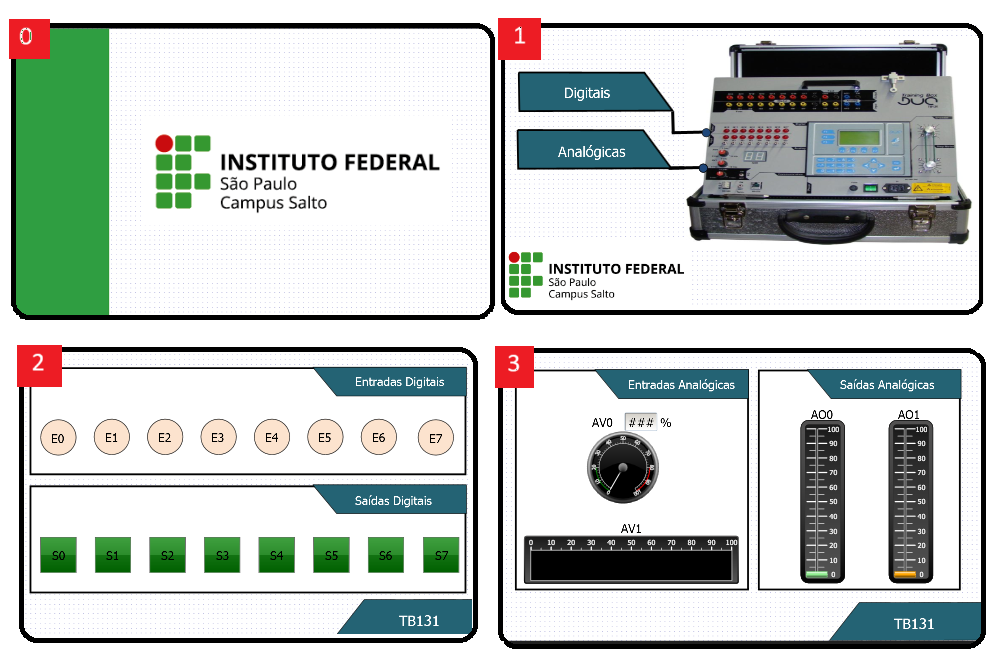
\includegraphics[width=14cm]{figuras/ativ1-telas}}
	}{
		\Fonte{Elaborado pelo autor}
	}
\end{figure}



Ao pressionar sobre o logo, ocorre a transição para a tela 1, que contem a ilustração do kit didático TB131 e as indicações dos dados analógicos e digitais. Essas indicações são botões para acesso aos dados respectivamente indicados.

Ao pressionar o botão \textbf{Digitais}, ocorre a transição para a tela 2, que contem um quadro com a indicação de \textbf{Entradas Digitais} e outro com a indicação de \textbf{Saídas Digitais}.

As entradas digitais são enumeradas de \textbf{E0} até \textbf{E7}, da mesma forma que no painal do TB131. 
Cada uma das entradas é um indicador que deve mostrar o estado lógico da respectiva entrada física do kit didático.

As saídas digitais são enumeradas de \textbf{S0} até \textbf{S7} e correspondem respectivamente às saídas \textbf{Q10} até \textbf{Q17} no painel do TB131. 
Cada uma das saídas é um botão que deve poder acionar a respectiva saída no kit didático, inclusive mudando a sua cor, indicando o estado lógico atual. 

Ao pressionar o botão no canto inferior direiro TB131, deve-se retornar à tela 1.

Ao pressionar o botão Analógicas, ocorre a transição para a tela 3, dividita também em dois quadros, um para as \textbf{Entradas Analógicas} e o outro para as \textbf{Saídas Analógicas}.

O quadro de entradas analógicas faz a leitura de duas variáveis analógicas do kit didático, associadas aos potenciômetros, AV0 e AV1. 
A variável \textbf{AV0} deve ser exibidas utilizando um \textbf{Display numérico} e um \textbf{Medidor Circular}, e a variável \textbf{AV1} deve ser exibida utilizando um \textbf{Medidor Linear} horizontal. 

Para as variáveis de saída, \textbf{AO0} e \textbf{AO1}, deve ser utilizado o componente \textbf{Slider}. 
No kit TB131, \textbf{AO0} pode ser visto através do display de 7 segmentos com dois dígitos, enquanto que o valor de \textbf{AO1} poderá ser medido com o auxílio de um multímetro entre os terminais \textbf{AO1} e \textbf{C4}. \textbf{C4} é o referencial, terra, da saída analógica \textbf{AO1}. 

Ao pressionar o botão no canto inferior direito TB131, deve-se retornar a tela 1.



